\documentclass[11pt]{article}
\usepackage[margin=1in]{geometry}
\usepackage[utf8]{inputenc}
\usepackage[T1]{fontenc}
\usepackage{lmodern}
\usepackage{amsmath,amssymb,amsthm}
\usepackage{tikz}
\usepackage{booktabs}
\usepackage{listings}
\usepackage{xcolor}
\usepackage{subcaption}
\usepackage{algorithm}
\usepackage{algorithmic}
\usepackage{hyperref}
\usetikzlibrary{positioning,calc,patterns,arrows.meta,shapes.geometric,shapes.symbols,fit,backgrounds,trees}
\newtheorem{theorem}{Theorem}
\newtheorem{remark}{Remark}
\newtheorem{example}{Example}
\lstdefinelanguage{Lean}{morekeywords={theorem,def,structure,inductive,where,match,with,by,fun,if,then,else,deriving,namespace,end,import},
  sensitive=true,morecomment=[l]{--},morecomment=[s]{/-}{-/},morestring=[b]"}
\lstdefinelanguage{CTR}{morekeywords={exec,run,var,decl,design,memory,program,end,COPY,NOT,INSIDE,OUTSIDE,ASSERT_ZERO},
  sensitive=true,morecomment=[l]{\#}}
\lstset{basicstyle=\ttfamily\small,keywordstyle=\color{blue!70!black},commentstyle=\color{green!40!black},
  frame=single,breaklines=true,columns=fullflexible,
  literate={∀}{{$\forall$}}1 {∃}{{$\exists$}}1 {↔}{{$\leftrightarrow$}}1 {→}{{$\to$}}1 {∈}{{$\in$}}1
           {¬}{{$\neg$}}1 {∧}{{$\wedge$}}1 {∨}{{$\vee$}}1 {₁}{{$_1$}}1 {₂}{{$_2$}}1 {⟨}{{$\langle$}}1
           {⟩}{{$\rangle$}}1 {σ}{{$\sigma$}}1 {≤}{{$\le$}}1 {×}{{$\times$}}1 {ρ}{{$\rho$}}1}
\newcommand{\op}[1]{\texttt{#1}}
\newcommand{\sel}[1]{\ensuremath{\mathsf{#1}}}
% shared TikZ styles
\tikzset{
  boxA/.style={draw=blue!70!black,thick,fill=blue!14},
  boxB/.style={draw=red!70!black,thick,dashed,fill=red!8,fill opacity=0.7},
  stage/.style={draw,rounded corners=3pt,thick,align=center,font=\small,minimum height=9mm,inner sep=4pt},
  file/.style={draw,thick,align=center,font=\small\ttfamily,minimum height=8mm,inner sep=3pt,
               tape,tape bend top=none,fill=yellow!10},
  flow/.style={-{Stealth[length=2.2mm]},thick},
  leaf/.style={draw,circle,thick,fill=gray!12,font=\scriptsize\ttfamily,minimum size=9mm,inner sep=0pt},
  keep/.style={draw,rounded corners=2pt,thick,fill=green!10,font=\scriptsize\ttfamily,minimum height=6mm,inner sep=2pt,align=center},
  gone/.style={draw=gray,rounded corners=2pt,dashed,fill=gray!8,text=gray,font=\scriptsize\ttfamily,minimum height=6mm,inner sep=2pt,align=center},
  copy/.style={draw=orange!80!black,rounded corners=2pt,thick,fill=orange!12,font=\scriptsize\ttfamily,minimum height=6mm,inner sep=2pt,align=center},
  use/.style={-{Stealth[length=1.6mm]},semithick},
  usegone/.style={-{Stealth[length=1.6mm]},gray!70,dashed},
  alias/.style={-{Stealth[length=1.8mm]},orange!80!black,very thick,densely dotted},
}
\title{Term Rewrite Synthesis for Boolean and 9E-DIM Layout Relations:\\
Engine-Faithful Semantics, Lean-Verified Completeness,\\ and a Compile-Time Optimizer in MAGPARSER}
\author{Sandeep Koranne}
\date{\today}
\begin{document}
\emergencystretch=3em
\maketitle

\begin{abstract}
We present a term rewrite synthesis (TRS) workflow for CTR layout programs that finds and removes operations whose result is provably empty, provably equal to an existing value, or idempotent. The relations come with Lean~4 proofs tied to the actual semantics of the layout engine. For geometric Booleans we prove that a $2^n$-row truth-table check is a sound and complete decision procedure for validity over all sets. For the topological (9E-DIM) selectors we transcribe the engine's box-level tests into Lean. Each pair of boxes falls into one of nine classes (Egenhofer's eight region relations, with \emph{meet} split by contact dimension), and we prove that every selector decision is a function of the set of classes a box has against the other layer. For healed layers exactly 14 class pairs are excluded, leaving 41 realizable types and 71 point types. This yields a sound and complete decision procedure for expressions mixing $A$, $B$, all 24 selectors $\sigma(A,B)$ and geometric Booleans. Size-bounded relation lists are characterized exactly by Lean theorems and kernel-checked counts, with no \texttt{sorry} and no \texttt{native\_decide}.
The 1{,}972 resulting rewrite rules are read from a text file by MAGPARSER itself: a Fortran DAG analyser and rewriter (\texttt{src/trs\_optimizer.f90}) optimizes every control file after m4 expansion and before execution. It agrees line by line with an independent Julia reference on 500 random programs, and every rule passes 59{,}250 engine assertions. Running optimized and original programs side by side exposed three subtleties, all handled by the rewriter: selectors read box decompositions, so geometric equality is not a congruence for them; and the engine's layer copy read freed memory when source and destination coincide, which corrupted both self-\op{COPY} and in-place operations such as \texttt{X = X NOT Y} (now fixed in the engine).
\end{abstract}

\section{Introduction}
CTR control files describe layout computations as a sequence of layer operations, e.g.\
\texttt{exec run m:r = d:diff * m:bna}. Programs generated by tools or written by hand often contain operations whose result is known in advance: $A\setminus A$, $A\cap(B\setminus A)$, or $(A\;\op{INSIDE}\;B)\cap(A\;\op{OUTSIDE}\;B)$. Removing them saves runtime. Doing so safely requires (i)~a precise semantics of each operator as the engine implements it, (ii)~proofs of the relations under that semantics, (iii)~an argument that the list of relations is complete in a well-defined sense, and (iv)~a rewriter that applies the relations without changing anything the engine computes. This paper supplies all four (Figure~\ref{fig:pipeline}):
\begin{itemize}
\item Section~\ref{sec:sem}: the engine semantics of Booleans and of the 24 box-level selectors.
\item Section~\ref{sec:lean}: Lean decision procedures and exactly characterized, size-bounded relation lists.
\item Section~\ref{sec:trs}: the compile-time optimizer inside MAGPARSER, its DAG model and its safety conditions.
\item Section~\ref{sec:val}: validation against the engine, including the engine defects the validation uncovered.
\end{itemize}
Section~\ref{sec:corrections} lists the errors of an earlier version of this work that the engine-faithful treatment corrects.

\begin{figure}[t]
\centering
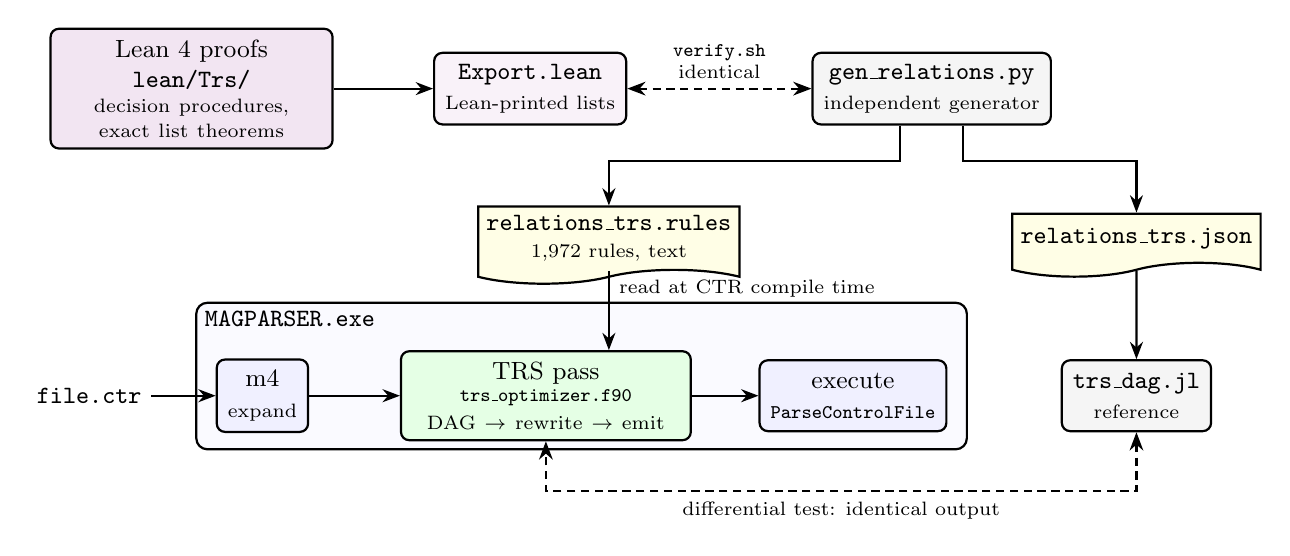
\begin{tikzpicture}[x=1cm,y=1cm]
\node[stage,fill=violet!10,text width=3.3cm] (lean) at (0,0) {Lean 4 proofs \texttt{lean/Trs/}\\[1pt]\scriptsize decision procedures,\\[-2pt]\scriptsize exact list theorems};
\node[stage,fill=violet!5] (exp) at (4.3,0) {\texttt{Export.lean}\\\scriptsize Lean-printed lists};
\node[stage,fill=gray!8] (py) at (9.4,0) {\texttt{gen\_relations.py}\\\scriptsize independent generator};
\draw[flow] (lean) -- (exp);
\draw[{Stealth}-{Stealth},thick,densely dashed] (exp) -- node[above,font=\scriptsize,align=center]{\texttt{verify.sh}\\identical} (py);
\node[file] (rules) at (5.3,-1.9) {relations\_trs.rules\\[-1pt]\scriptsize\rmfamily 1{,}972 rules, text};
\node[file] (json) at (12.0,-1.9) {relations\_trs.json};
\draw[flow] (py.south) ++(-0.4,0) |- ++(0,-0.45) -| (rules.north);
\draw[flow] (py.south) ++(0.4,0) |- ++(0,-0.45) -| (json.north);
\node[stage,fill=blue!6] (m4) at (0.9,-3.9) {m4\\\scriptsize expand};
\node[stage,fill=green!10,text width=3.4cm] (trs) at (4.5,-3.9) {TRS pass\\\scriptsize\texttt{trs\_optimizer.f90}\\[-1pt]\scriptsize DAG $\to$ rewrite $\to$ emit};
\node[stage,fill=blue!6] (exe) at (8.4,-3.9) {execute\\\scriptsize\texttt{ParseControlFile}};
\node[font=\small\ttfamily] (ctr) at (-1.3,-3.9) {file.ctr};
\draw[flow] (ctr) -- (m4); \draw[flow] (m4) -- (trs); \draw[flow] (trs) -- (exe);
\begin{scope}[on background layer]
\node[draw,thick,rounded corners=4pt,fill=blue!2,fit=(m4)(trs)(exe),inner sep=7pt,yshift=2.5mm,inner ysep=10pt] (mag) {};
\end{scope}
\node[font=\small\bfseries,anchor=north west] at (mag.north west) {\texttt{MAGPARSER.exe}};
\draw[flow] (rules.south) -- (rules.south |- trs.north) node[pos=0.22,right,font=\scriptsize]{read at CTR compile time};
\node[stage,fill=gray!8] (jl) at (12.0,-3.9) {\texttt{trs\_dag.jl}\\\scriptsize reference};
\draw[flow] (json) -- (jl);
\draw[{Stealth}-{Stealth},thick,densely dashed] (jl.south) -- ++(0,-0.75) -| node[pos=0.25,below,font=\scriptsize]{differential test: identical output} (trs.south);
\end{tikzpicture}
\caption{Workflow. Lean proves the relations and prints the lists; an independent Python generator must agree line by line. The rules are exported as a text file that MAGPARSER reads when it compiles a control file: after m4 expansion and before execution, the Fortran TRS pass builds the operation DAG, rewrites it and emits the optimized control file that is then executed. The Julia tool is an independent reference implementation of the same rewriter.}
\label{fig:pipeline}
\end{figure}

\section{Engine semantics}\label{sec:sem}
\subsection{Geometric Booleans}
The CTR operators \op{*}/\op{AND2} (intersection), \op{+}/\op{OR2} (union), \op{NOT}/\op{@}/\op{!} (difference $A\setminus B$) and \op{XOR}/\op{\^{}} (symmetric difference) act on regions. Results are regularized: zero-area pieces are dropped. With integer coordinates we use \emph{cells}, i.e.\ unit squares $[c_x,c_x{+}1]\times[c_y,c_y{+}1]$. Two regions are equal up to measure zero iff they contain the same cells, so ``pointwise'' below means ``cellwise''.

\begin{remark}
The CTR keyword \op{AND} is \emph{not} intersection. It calls \texttt{CalculateSingleLayerAND(rhs1)}, which ignores the second operand and computes the self-overlap of one layer. CTR has no unary complement either. A complement exists only relative to an \op{EXTENT} universe.
\end{remark}

\subsection{Topological selectors}
\texttt{CalculateTopologicalSelect} (\texttt{src/design\_topo\_impl.f90}) first heals both operands into non-degenerate boxes with pairwise-disjoint interiors. It then keeps or drops each \emph{whole box} $a$ of $A$ according to how $a$ relates to the individual boxes $b$ of $B$. Comparing $a$ with one $b$ yields exactly one of nine classes (Figure~\ref{fig:classes}). The \emph{type} of $a$ is the set of non-disjoint classes it has against $B$. Table~\ref{tab:sel} gives each selector as a predicate on types. Lean proves that these predicates are exactly what the Fortran code computes (Theorem~\ref{thm:sel}).

\begin{figure}[t]
\centering
\newcommand{\cls}[4]{\begin{scope}[shift={(#1,#2)}]#3
  \node[font=\small\bfseries,anchor=north] at (1.1,-0.2){#4};\end{scope}}
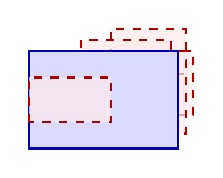
\begin{tikzpicture}[scale=0.95]
\cls{0}{2.6}{\draw[boxA](0,0)rectangle(1,1);\draw[boxB](1.35,0.45)rectangle(2.2,1.3);}{DISJ}
\cls{3}{2.6}{\draw[boxA](0,0)rectangle(1.1,1);\draw[boxB](1.1,1)rectangle(2.1,1.6);\fill[black](1.1,1)circle(1.6pt);}{PT}
\cls{6}{2.6}{\draw[boxA](0,0)rectangle(1.1,1);\draw[boxB](1.1,0.2)rectangle(2.1,1.3);\draw[black,ultra thick](1.1,0.2)--(1.1,1);}{ET}
\cls{9}{2.6}{\draw[boxA](0,0)rectangle(1.2,1);\draw[boxB](0.7,0.45)rectangle(1.9,1.45);}{PO}
\cls{12}{2.6}{\draw[boxA](0.3,0)rectangle(1.8,1.1);\draw[boxB](0.3,0)rectangle(1.8,1.1);}{EQ}
\cls{1.5}{0}{\draw[boxB](0,0)rectangle(2,1.3);\draw[boxA](0.5,0.35)rectangle(1.4,0.95);}{INS}
\cls{4.8}{0}{\draw[boxB](0,0)rectangle(2,1.3);\draw[boxA](0,0.35)rectangle(1.1,0.95);}{INB}
\cls{8.1}{0}{\draw[boxA](0,0)rectangle(2,1.3);\draw[boxB](0.5,0.35)rectangle(1.4,0.95);}{CONS}
\cls{11.4}{0}{\draw[boxA](0,0)rectangle(2,1.3);\draw[boxB](0,0.35)rectangle(1.1,0.95);}{CONB}
\end{tikzpicture}
\caption{The nine pairwise classes of an $A$ box (solid blue) against a $B$ box (dashed red). Top: disjoint, point (corner) contact, edge contact, proper overlap, equal. Bottom: inside without/with a shared boundary coordinate, contains without/with a shared boundary coordinate. These are Egenhofer's eight region relations with \emph{meet} split into PT and ET by contact dimension.}
\label{fig:classes}
\end{figure}

\begin{table}[t]
\centering\small
\begin{tabular}{ll}
\toprule
selector & box $a$ of $A$ is kept iff its type \dots\\
\midrule
\op{INTERACT} & contains an overlap class (PO, EQ, INS, INB, CONS, CONB)\\
\op{INSIDE} & contains EQ, INS or INB ($a$ lies inside \emph{one} $B$ box)\\
\op{OUTSIDE}, \op{DISJOINT} & is empty (no contact at all); the two are identical\\
\op{TOUCH} & contains ET and no overlap class\\
\op{MEET} & contains PT or ET and no overlap class\\
\op{CUT} & contains an overlap class but not EQ/INS/INB\\
\op{EQUAL} & contains EQ\\
\op{CONTAINS} / \op{COVERS} & contains EQ, CONS or CONB / EQ or CONB\\
\op{COVEREDBY} & contains EQ or INB\\
\op{OVERLAPS} & contains PO\\
\op{NOT\_}$X$ & complement of $X$ within $A$'s boxes\\
\bottomrule
\end{tabular}
\caption{Selectors as predicates on box types (\texttt{Trs.Box.basePred}).}
\label{tab:sel}
\end{table}

Consequences: $A\;\op{INSIDE}\;B \neq A\cap B$, since a box of $A$ that straddles two $B$ boxes is dropped, and \op{CONTAINS} keeps boxes that extend beyond $B$. In general a selector's result depends on box decompositions, not only on geometry (Figure~\ref{fig:decomp}). This single fact drives most of the safety conditions of Section~\ref{sec:trs}.

\begin{figure}[t]
\centering
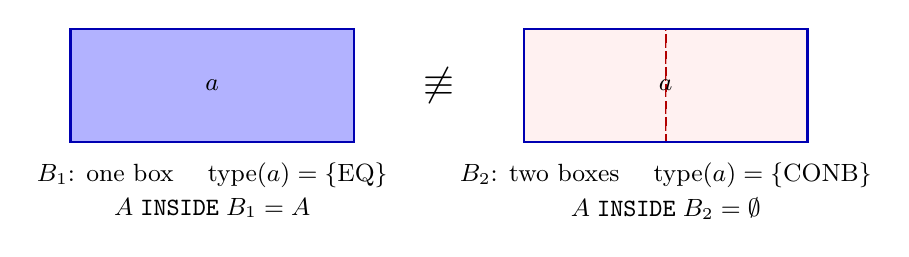
\begin{tikzpicture}[scale=0.9]
\begin{scope}
  \draw[boxB] (0,0) rectangle (4,1.6);
  \draw[boxA,fill=blue!30] (0,0) rectangle (4,1.6);
  \node[font=\small] at (2,0.8) {$a$};
  \node[font=\small,anchor=north] at (2,-0.15) {$B_1$: one box \quad type$(a)=\{\mathrm{EQ}\}$};
  \node[font=\small,anchor=north] at (2,-0.65) {$A\;\op{INSIDE}\;B_1 = A$};
\end{scope}
\node[font=\Large] at (5.2,0.8) {$\not\equiv$};
\begin{scope}[xshift=6.4cm]
  \draw[boxB] (0,0) rectangle (2,1.6); \draw[boxB] (2,0) rectangle (4,1.6);
  \draw[draw=blue!70!black,thick] (0,0) rectangle (4,1.6);
  \node[font=\small] at (2,0.8) {$a$};
  \node[font=\small,anchor=north] at (2,-0.15) {$B_2$: two boxes \quad type$(a)=\{\mathrm{CONB}\}$};
  \node[font=\small,anchor=north] at (2,-0.65) {$A\;\op{INSIDE}\;B_2 = \emptyset$};
\end{scope}
\end{tikzpicture}
\caption{Geometry is not enough. $B_1$ and $B_2$ cover exactly the same cells, yet $A\;\op{INSIDE}\;B$ keeps the box $a$ for $B_1$ (class EQ) and drops it for $B_2$ (against each half, $a$ is in class CONB, and no single $B$ box contains $a$). A rewrite that replaces $B_1$ by a geometrically equal value with the decomposition of $B_2$ changes every later selector that reads it.}
\label{fig:decomp}
\end{figure}

\section{Lean development}\label{sec:lean}
The development (\texttt{lean/Trs/}, Lean 4.36.0, core only) has four parts.

\subsection{Boolean completeness}
\begin{lstlisting}[language=Lean]
def Valid (e₁ e₂ : Expr n) : Prop :=
  ∀ (U : Type) (L : Fin n → U → Prop) (u : U), e₁.evalSet L u ↔ e₂.evalSet L u
theorem valid_iff_bool   : Valid e₁ e₂ ↔ ∀ ρ : Fin n → Bool, e₁.eval ρ = e₂.eval ρ
theorem valid_iff_decide : Valid e₁ e₂ ↔ decideEquiv e₁ e₂ = true
\end{lstlisting}
\begin{theorem}[Boolean decision procedure]
An identity between layer expressions over $n$ layers holds for all subsets of every universe iff it holds on all $2^n$ Bool assignments. The truth-table check \texttt{decideEquiv} decides this exactly. In particular, no valid Boolean relation can be missed.
\end{theorem}

\subsection{Selectors are functions of the type}
\texttt{cls\_spec} gives the coordinate meaning of each class. \texttt{pf\_eq} shows that each per-pair sub-predicate in the Fortran loop is a function of the class. \texttt{flag\_eq} lifts this to whole layers.
\begin{lstlisting}[language=Lean]
theorem engineSel_eq (op : Op) (a : Box) (B : List Box) (ha : a.ok)
    (hB : ∀ b ∈ B, b.ok = true) : engineSel op a B = selPred op (tyOf a B)
\end{lstlisting}
\begin{theorem}\label{thm:sel}
For every selector (12 base relations, plus their negations) and every non-degenerate box $a$ and layer $B$, the engine's decision for $a$ equals the Table~\ref{tab:sel} predicate applied to the type of $a$.
\end{theorem}

\subsection{Healed layers and point types}
\begin{theorem}[Realizability]\label{thm:real}
If $B$ is healed, the type of any box avoids the 14 class pairs of Table~\ref{tab:forb} (\texttt{pair\_compat}, \texttt{tyOf\_realizable}). Every type that avoids them occurs (witnesses below). This leaves 41 of the 256 possible types.
\end{theorem}
\begin{table}[h]
\centering\small
\begin{tabular}{ll}
\toprule
class & cannot co-occur (healed $B$) with\\
\midrule
EQ & PO, INS, INB, CONS, CONB\\
INS & PT, ET, PO, INB, CONS, CONB \quad (an INS box has type exactly \{INS\})\\
INB & PO, CONS, CONB\\
\bottomrule
\end{tabular}
\caption{Forbidden class pairs, each proved geometrically by \texttt{omega}.}
\label{tab:forb}
\end{table}
A cell sees a \emph{point type} $(m_A, m_B, t)$: whether it is in $A$, whether it is in $B$, and the type of the unique $A$ box containing it (\texttt{cell\_unique}). Valid point types satisfy: $t$ is realizable; \textbf{C1}: if $t$ contains EQ, INS or INB then $m_B$ holds; \textbf{C2}: if $m_B$ holds then $t$ contains an overlap class. Exactly 71 point types are valid (\texttt{validPTs\_length}).

\begin{lstlisting}[language=Lean]
theorem cellEval_eq (hA : healedB A = true) (hB : ∀ b ∈ B, b.ok = true) (e : MExpr) :
    cellEval A B c e = ptEval (ptOf A B c) e
theorem complete (e₁ e₂ : MExpr) : HealedValid e₁ e₂ ↔ decideM e₁ e₂ = true
\end{lstlisting}
\begin{theorem}[9E-DIM decision procedure]\label{thm:complete}
Let $e_1,e_2$ be expressions built from $A$, $B$, the 24 selectors $\sigma(A,B)$ and geometric Booleans. Then $e_1$ and $e_2$ agree at every cell of every healed configuration iff they agree on the 71 valid point types. Soundness follows from \texttt{ptOf\_valid} and \texttt{cellEval\_eq}. For completeness, a generated table supplies one concrete healed configuration per point type, and the kernel checks every entry (\texttt{witOk\_all}).
\end{theorem}
Selector outputs keep $A$'s boxes, and the engine does not re-heal them. Lean therefore proves the box-list identity $\sigma_2(\sigma_1(A,B),B) = A\,|\,\sigma_1\wedge\sigma_2$ (\texttt{nest\_eq}) and, cellwise, idempotence $\sigma(\sigma(A,B),B)=\sigma(A,B)$ (\texttt{sel\_idem}).

\subsection{Complete lists}
A list of identities is infinite, so the lists are complete \emph{up to a size bound}. Lean enumerates every term up to the bound (\texttt{termsUpTo}, \texttt{mtermsUpTo}) and filters it with the proven decision procedure. \texttt{zeroTerms\_spec}, \texttt{inputTerms\_sound/complete}, \texttt{mzeroTerms\_spec} and \texttt{matomTerms\_sound/complete} state that each list is \emph{exactly} the set of bounded terms with that property. The kernel checks the counts in Table~\ref{tab:counts}. \texttt{RELATIONS.md} is printed from the same Lean definitions. An independent Python implementation produces identical lists line by line (\texttt{trs/verify.sh}).

\begin{table}[h]
\centering\small
\begin{tabular}{llrrrr}
\toprule
model & atoms & size $\le$ & terms & $E=0$ & $E=$ atom\\
\midrule
Boolean & 2 layers & 3 & 5{,}394 & 1{,}306 & 1{,}572\\
Boolean & 3 layers & 3 & 26{,}823 & 4{,}176 & 4{,}986\\
Boolean & 4 layers & 3 & 84{,}036 & 9{,}532 & 11{,}272\\
9E-DIM & $A$, $B$, 24 selectors & 1 & 2{,}730 & 353 & 1{,}283\\
9E-DIM & $A$, $B$, 24 selectors & 2 & 565{,}162 & 86{,}064 & 254{,}957$^\dagger$\\
\bottomrule
\end{tabular}
\caption{Exhaustive relation counts. Size is the number of binary operators. The Boolean lists use only CTR-expressible operators. All counts except $^\dagger$ are kernel-checked; $^\dagger$ was computed by Lean evaluation and independently by Python. The only coincidences among the 26 atoms are $\op{DISJOINT}=\op{OUTSIDE}$ and its negation.}
\label{tab:counts}
\end{table}

Of the 353 size-1 zero relations, 16 genuinely need $B$ to be healed (e.g.\ $(A\;\op{INSIDE}\;B)\cap(A\;\op{OVERLAPS}\;B)=0$). The other 337 also hold if every one of the 256 types is allowed (a Python observation, not proved in Lean).

\section{Sixteen verified ALL\_ZERO relations}
Figure~\ref{fig:allzero} shows sixteen relations taken from the verified lists. The Boolean entries (top two rows) hold in every set model. The selector entries (bottom two rows) hold for healed layers in the engine semantics; there \sel{IN}, \sel{OUT}, \dots\ abbreviate $A\;\op{INSIDE}\;B$, $A\;\op{OUTSIDE}\;B$, \dots

\begin{figure}[p]
\centering
% Boolean rows: A = [0,1.5]x[0,1], B = [0.8,2.3]x[0.15,0.85]; P (blue) and Q (red) are the two operands
\tikzset{P/.style={fill=blue!45,fill opacity=0.6},Q/.style={pattern=north east lines,pattern color=red!80!black}}
\newcommand{\frameAB}{\draw[thick] (0,0) rectangle (1.5,1); \draw[thick,dashed] (0.8,0.15) rectangle (2.3,0.85); \node[font=\tiny,anchor=north west] at (0,1){$A$}; \node[font=\tiny,anchor=north east] at (2.3,0.85){$B$};}
\newcommand{\rA}{(0,0) rectangle (1.5,1)}
\newcommand{\rB}{(0.8,0.15) rectangle (2.3,0.85)}
\newcommand{\rAB}{(0.8,0.15) rectangle (1.5,0.85)}
\newcommand{\rAmB}{(0,0) rectangle (0.8,1) (0.8,0) rectangle (1.5,0.15) (0.8,0.85) rectangle (1.5,1)}
\newcommand{\rBmA}{(1.5,0.15) rectangle (2.3,0.85)}
% Selector rows: healed B = b1 [0.9,1.8]x[0.1,0.9], b2 [1.8,2.2]x[0.3,0.7];
% A boxes: in (INS), eq (=b2), cut (PO), tch (ET), out (far)
\newcommand{\frameSel}{\draw[thick,dashed] (0.9,0.1) rectangle (1.8,0.9); \draw[thick,dashed] (1.8,0.3) rectangle (2.2,0.7);
  \draw[thick] (1.1,0.3) rectangle (1.5,0.7); \draw[thick] (1.8,0.3) rectangle (2.2,0.7);
  \draw[thick] (0.6,0.5) rectangle (1.0,0.8); \draw[thick] (0.5,0.1) rectangle (0.9,0.35);
  \draw[thick] (0.05,0.1) rectangle (0.4,0.4);
  \node[font=\tiny,anchor=south east] at (2.2,0.9){$B$};}
\newcommand{\sIn}{(1.1,0.3) rectangle (1.5,0.7) (1.8,0.3) rectangle (2.2,0.7)}
\newcommand{\sEq}{(1.8,0.3) rectangle (2.2,0.7)}
\newcommand{\sCut}{(0.6,0.5) rectangle (1.0,0.8)}
\newcommand{\sTch}{(0.5,0.1) rectangle (0.9,0.35)}
\newcommand{\sOut}{(0.05,0.1) rectangle (0.4,0.4)}
\newcommand{\sB}{(0.9,0.1) rectangle (1.8,0.9) (1.8,0.3) rectangle (2.2,0.7)}
\newcommand{\cellX}[4]{\begin{minipage}[t]{0.24\textwidth}\centering
  \begin{tikzpicture}[scale=1.3]#1#4\end{tikzpicture}\\[2pt]
  {\small #2}\\[1pt]{\scriptsize\color{black!65}#3}\end{minipage}}
\newcommand{\cellB}[3]{\cellX{#1}{#2}{#3}{\frameAB}}
\newcommand{\cellS}[3]{\cellX{#1}{#2}{#3}{\frameSel}}
\cellB{\fill[P]\rA;}{$A\setminus A=0$}{blue: $A$ (both operands)}\hfill
\cellB{\fill[P]\rA; \fill[Q]\rBmA;}{$A\cap(B\setminus A)=0$}{blue $A$, red $B\setminus A$}\hfill
\cellB{\fill[P]\rAB; \fill[Q]\rA;}{$(A\cap B)\setminus A=0$}{blue $A\cap B$ inside red $A$}\hfill
\cellB{\fill[P]\rA;}{$A\oplus A=0$}{blue: $A$ (both operands)}

\vspace{0.9em}
\cellB{\fill[P]\rAB; \fill[Q]\rAmB;}{$(A\cap B)\cap(A\setminus B)=0$}{blue $A\cap B$, red $A\setminus B$}\hfill
\cellB{\fill[P]\rA; \fill[P]\rB;}{$(A\cup B)\setminus(A\cup B)=0$}{blue: $A\cup B$ (both)}\hfill
\cellB{\fill[P]\rAB; \fill[Q]\rAmB; \fill[Q]\rBmA;}{$(A\oplus B)\cap(A\cap B)=0$}{red $A\oplus B$, blue $A\cap B$}\hfill
\cellB{\fill[P]\rAmB; \fill[Q]\rB;}{$(A\setminus B)\cap B=0$}{blue $A\setminus B$, red $B$}

\vspace{0.9em}
\cellS{\fill[P]\sIn; \fill[Q]\sOut;}{$\sel{IN}\cap\sel{OUT}=0$}{blue \sel{IN}, red \sel{OUT}}\hfill
\cellS{\fill[Q]\sB; \fill[P]\sIn;}{$\sel{IN}\setminus B=0$}{blue \sel{IN} inside red $B$}\hfill
\cellS{\fill[P]\sOut; \fill[Q]\sB;}{$\sel{OUT}\cap B=0$}{blue \sel{OUT}, red $B$}\hfill
\cellS{\fill[P]\sTch; \fill[Q]\sOut;}{$\sel{MEET}\cap\sel{DISJOINT}=0$}{blue \sel{MEET}, red \sel{DISJOINT}}

\vspace{0.9em}
\cellS{\fill[P]\sEq; \fill[Q]\sCut;}{$\sel{EQUAL}\cap\sel{OVERLAPS}=0^\ast$}{blue \sel{EQUAL}, red \sel{OVERLAPS}}\hfill
\cellS{\fill[P]\sIn; \fill[Q]\sCut;}{$\sel{IN}\cap\sel{OVERLAPS}=0^\ast$}{blue \sel{IN}, red \sel{OVERLAPS}}\hfill
\cellS{\fill[P]\sTch; \fill[Q]\sB;}{$\sel{TOUCH}\cap B=0$}{blue \sel{TOUCH}, red $B$}\hfill
\cellS{\fill[Q]\sCut; \fill[P]\sIn;}{$\sel{CUT}\cap\sel{IN}=0$}{red \sel{CUT}, blue \sel{IN}}
\caption{Sixteen relations that are empty by construction, all members of the Lean-characterized lists. Each panel colors the two operands of the outermost operation (blue solid, red hatched): they are disjoint, or the first lies inside the subtracted operand. Rows 1--2: regions $A$ (solid outline) and $B$ (dashed). Rows 3--4: one healed configuration with $B$ = two dashed boxes and five $A$ boxes (inside, equal to a $B$ box, cutting, edge-touching, far away). $^\ast$: requires $B$ healed, which the engine guarantees. Relations such as $\sel{IN}\oplus(A\cap B)=0$ or $\sel{CONTAINS}\setminus B=0$ are \emph{not} valid; the decision procedure rejects them.}
\label{fig:allzero}
\end{figure}

Selected identities that equal an input or are idempotent (all in the lists): $A\cap A=A$, $A\cup A=A$, $(A\cap B)\cup A=A$, $((A\oplus B)\oplus A)=B$, $\sel{IN}\cap A=\sel{IN}$, $\sel{IN}\cup\sel{NOT\_IN}=A$, $\sel{MEET}\oplus A=\sel{NOT\_MEET}$, and $\sigma(\sigma(A,B),B)=\sigma(A,B)$ for every selector $\sigma$.

%======================================================================
\section{The compile-time TRS optimizer in MAGPARSER}\label{sec:trs}
The rewriter is a Fortran module, \texttt{TRSOptimizerModule} in \texttt{src/trs\_optimizer.f90}, linked into \texttt{MAGPARSER.exe}. \texttt{ParseControlFile} expands the control file with m4 as before. If a rules file is configured, it then calls \texttt{TRSOptimizeFile} on the expanded file, prints the optimized program and executes that program instead (Figure~\ref{fig:pipeline}). Because optimization happens when the control file is compiled, before any layer is loaded, it costs milliseconds and needs no geometry. The same module is also built as a stand-alone tool, \texttt{TRS\_OPT.exe rules in.ctr out.ctr}.

\subsection{Enabling it}
\begin{lstlisting}[language=CTR]
program demo
var trs_rules /path/to/relations_trs.rules   # or: export MAGPARSER_TRS_RULES=...
var temporary_layers 2
decl design d = chip.mag
decl memory m = nothing
var trs_enable 0          # freeze a region: no rewrites, no removals
exec run m:ref = d:diff NOT d:diff
var trs_enable 1
exec run m:r1 = d:diff NOT d:diff                    # removed: provably empty
end
\end{lstlisting}
A \texttt{var trs\_rules} line in the file takes precedence over the environment variable; the values \texttt{none}/\texttt{off} disable the pass for one file. \texttt{var trs\_enable 0}/\texttt{1} brackets a frozen region, which the engine-level test of Section~\ref{sec:val} uses to keep a reference copy of a program untouched. The rules file is plain text, one rule per line, generated from the Lean-checked lists by \texttt{trs/gen\_relations.py}:
\begin{lstlisting}
TRS_RULES 1 1972
bool_zero_15 | zero | (A * (B NOT A)) | 0 | Trs.Bool.zeroTerms 3 3 (zeroTerms_spec)
box_zero_22  | zero | ((A INSIDE B) NOT B) | 0 | Trs.Box.mzeroTerms 1 (mzeroTerms_spec)
bool_input_141 | atom | ((A ^ B) ^ A) | B | Trs.Bool.inputTerms 3 3 (inputTerms_sound)
\end{lstlisting}
The fields are name, kind, a fully parenthesized left-hand side over the pattern variables $A,B,C$, the right-hand side ($0$, a variable or sub-pattern of the left side, or one selector over two variables), and the Lean definition and theorem that justify the rule. Of the 1{,}972 rules, 479 rewrite to the empty layer and 1{,}493 to an existing value or a single selector.

\subsection{The DAG}
Each \texttt{exec run} line becomes a node whose operator follows the parser of \texttt{controlparser.f90}: single-character operators are recognized first, then \op{AND2}, \op{OR2}, \op{NOT}, \op{XOR}, the 24 selectors (also written \op{NOT INSIDE}), and every edge operator or unknown keyword, including the single-layer \op{AND}, is \emph{opaque}. Operands are resolved by \emph{reaching definition}: a hash map from layer name to the node that currently defines it. A name that is redefined later therefore still refers to the earlier value (Example~\ref{ex:redef}). For each node the pass records the line of the next redefinition of its name. A value $v$ can be referred to by name at line $\ell$ iff it was defined before $\ell$ and its name is not redefined before $\ell$. This test is $O(1)$. A reverse adjacency (``users'') graph supports the reachability test below. Alias edges are added as COPY rewrites are made.

\begin{example}[reaching definitions]\label{ex:redef}
In \texttt{example\_trs\_redef.ctr}, \texttt{m:t = d:poly * d:diff} is followed by \texttt{m:r = d:diff * m:t} and only then by \texttt{m:t = d:poly NOT d:diff}. The rule $A\cap(B\setminus A)=0$ matches \texttt{m:s = d:diff * m:t} (second \texttt{m:t}) but not \texttt{m:r}, whose operand is the first \texttt{m:t}. A ``last definition'' lookup, as in the earlier version of this tool, rewrites the non-empty \texttt{m:r} to $0$.
\end{example}

\subsection{Rewriting}
Nodes are visited in program order (Algorithm~\ref{alg:trs}). A rule matches a node when the left-hand side unifies with the sub-DAG below it. Matching sees through COPY aliases, uses only live (unrewritten) nodes outside connectivity zones, and binds repeated variables to the same value. Each rewrite turns a node into the empty layer, a COPY of an existing value, or a single selector over existing values. Every rewrite therefore removes at least one operation, and the pass terminates after one sweep. Empty results are propagated: $X\cap 0=0$, $X\cup0=X$, $X\setminus0=X$, $0\setminus X=0$, and a selector with an empty $A$ is empty. With an empty $B$ the selector follows the engine's \texttt{numB}$=0$ branch, which keeps all of $A$ for the twelve ``negative'' selectors (\op{OUTSIDE}, \op{DISJOINT}, \op{NOT\_INTERACT}, \dots) and drops all of it otherwise. Finally, a node is deleted when its value is provably empty or it has become an orphaned memory temporary, provided no kept line still uses its value. The deletion is iterated to a fixpoint. A provably empty value that is still used is kept and annotated.

\begin{algorithm}[t]
\caption{TRS pass (\texttt{TRSOptimizeFile})}\label{alg:trs}
\begin{algorithmic}[1]
\STATE parse rules; parse CTR into nodes with reaching-definition operands, zones, frozen flags
\FOR{each node $n$ in program order, not opaque, not in a zone, not frozen}
  \IF{an operand of $n$ is empty} \STATE fold $n$ (empty propagation, engine empty-$B$ branch)
  \ELSIF{$n=\sigma(\sigma(A,B),B)$} \STATE alias $n\mapsto\sigma(A,B)$ \hfill (\texttt{nest\_eq}: equal box lists)
  \ELSE
    \FOR{each rule $l\to r$ in file order}
      \IF{$l$ matches at $n$ \AND the rewrite is \emph{safe} (below)}
        \STATE $n \gets 0$, or alias $n\mapsto r$, or replace $n$ by the selector $r$; \textbf{break}
      \ENDIF
    \ENDFOR
  \ENDIF
\ENDFOR
\STATE delete empty/orphaned memory nodes not used by kept lines (fixpoint); emit annotated CTR
\end{algorithmic}
\end{algorithm}

\subsection{Safety conditions}
The Lean relations are cellwise equalities, which is weaker than what the engine observes. A rewrite to a non-empty value is applied only if all of the following hold:
\begin{enumerate}
\item \textbf{Nameable.} The target value can be named at the line (no intervening redefinition).
\item \textbf{No selector downstream.} The node's value cannot reach a selector operand through any chain of later operations, including COPY aliases (\texttt{feeds\_selector}). Figure~\ref{fig:decomp} shows why: a geometrically equal value with another box decomposition changes a later selector. The empty layer has no boxes, so rewrites to $0$ are always safe. The nesting rule is an equality of box lists, so it is safe everywhere.
\item \textbf{Zones.} Nothing inside \texttt{START/END CONNECT ZONE} is rewritten, and no COPY is introduced for a value consumed inside a zone. A COPY may carry a different net-id (Section~\ref{sec:conn}).
\item \textbf{No self-COPY.} If the target is still held by the node's own name, then the line is deleted instead of emitting \texttt{X = X COPY nothing} (Figure~\ref{fig:selfcopy}).
\item \textbf{No in-place operation.} A selector replacement is not emitted if its output name equals one of its operand names.
\end{enumerate}
Conditions 4 and 5 were added after the engine-level test found that the engine mishandled these forms (Section~\ref{sec:issues}). The engine is now fixed, and the conditions keep the optimizer safe with older builds.

\begin{figure}[t]
\centering
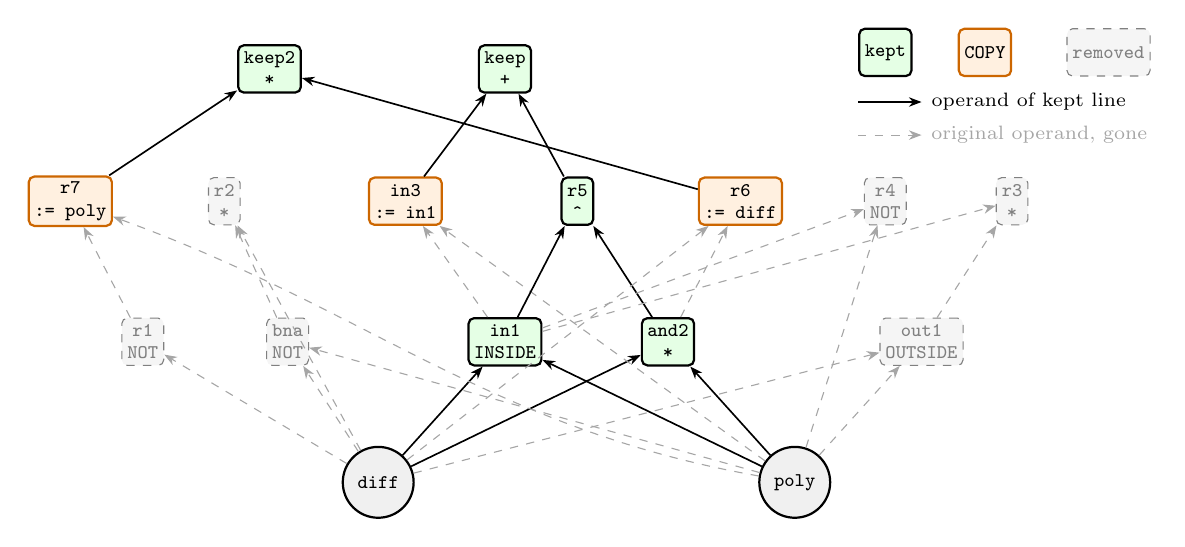
\begin{tikzpicture}[x=1.15cm,y=1.05cm]
\node[leaf] (A) at (3,0) {diff}; \node[leaf] (B) at (7.6,0) {poly};
% level 1
\node[gone] (r1)   at (0.4,1.7) {r1\\NOT};
\node[gone] (bna)  at (2.0,1.7) {bna\\NOT};
\node[keep] (in1)  at (4.4,1.7) {in1\\INSIDE};
\node[keep] (and2) at (6.2,1.7) {and2\\*};
\node[gone] (out1) at (9.0,1.7) {out1\\OUTSIDE};
% level 2
\node[copy] (r7)   at (-0.4,3.4) {r7\\:= poly};
\node[gone] (r2)   at (1.3,3.4) {r2\\*};
\node[copy] (in3)  at (3.3,3.4) {in3\\:= in1};
\node[keep] (r5)   at (5.2,3.4) {r5\\\^{}};
\node[copy] (r6)   at (7.0,3.4) {r6\\:= diff};
\node[gone] (r4)   at (8.6,3.4) {r4\\NOT};
\node[gone] (r3)   at (10.0,3.4) {r3\\*};
% level 3
\node[keep] (k2) at (1.8,5.0) {keep2\\*};
\node[keep] (k1) at (4.4,5.0) {keep\\+};
% edges (operand -> user)
\draw[usegone] (A) -- (r1); \draw[usegone] (A) -- (bna); \draw[usegone] (B) -- (bna);
\draw[use] (A) -- (in1); \draw[use] (B) -- (in1);
\draw[use] (A) -- (and2); \draw[use] (B) -- (and2);
\draw[usegone] (A) -- (out1); \draw[usegone] (B) -- (out1);
\draw[usegone] (r1) -- (r7); \draw[usegone] (B) to[out=170,in=-20] (r7);
\draw[usegone] (A) -- (r2); \draw[usegone] (bna) -- (r2);
\draw[usegone] (in1) -- (in3); \draw[usegone] (B) -- (in3);
\draw[use] (in1) -- (r5); \draw[use] (and2) -- (r5);
\draw[usegone] (and2) -- (r6); \draw[usegone] (A) -- (r6);
\draw[usegone] (in1) -- (r4); \draw[usegone] (B) -- (r4);
\draw[usegone] (in1) -- (r3); \draw[usegone] (out1) -- (r3);
\draw[use] (r7) -- (k2); \draw[use] (r6) -- (k2);
\draw[use] (r5) -- (k1); \draw[use] (in3) -- (k1);
% legend
\begin{scope}[shift={(8.3,5.2)}]
\node[keep,anchor=west] at (0,0) {kept};
\node[copy,anchor=west] at (1.1,0) {COPY};
\node[gone,anchor=west] at (2.3,0) {removed};
\draw[use] (0,-0.6) -- (0.7,-0.6) node[right,font=\scriptsize]{operand of kept line};
\draw[usegone] (0,-1.0) -- (0.7,-1.0) node[right,font=\scriptsize]{original operand, gone};
\end{scope}
\end{tikzpicture}
\caption{The DAG of \texttt{example\_trs.ctr} after the TRS pass; edges run from operands up to their users, and ``$x$ := $y$'' marks a node emitted as \texttt{x = y COPY nothing}. \texttt{r1}, \texttt{r2}, \texttt{r3}, \texttt{r4} are provably empty (\texttt{bool\_zero\_0}, \texttt{bool\_zero\_15}, \texttt{box\_zero\_26}, \texttt{box\_zero\_22}). \texttt{bna} and \texttt{out1} then become orphans and are removed too. \texttt{in3} $=\sigma(\sigma(A,B),B)$ aliases \texttt{in1} (\texttt{nest\_eq}, safe even though \texttt{in1} feeds a selector), \texttt{r6} $=(A\cap B)\cup A$ aliases \texttt{diff} (\texttt{bool\_input\_136}), and \texttt{r7} $=B\cup 0$ aliases \texttt{poly}. \texttt{r5} $=\sel{IN}\oplus(A\cap B)$ is \emph{not} a valid identity and stays. Result: 14 operations become 8, three of which are COPYs.}
\label{fig:dag}
\end{figure}

\begin{figure}[t]
\centering
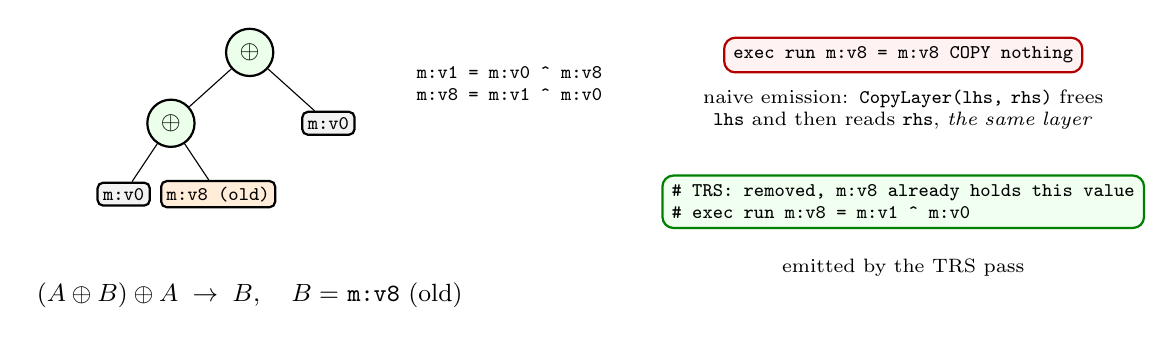
\begin{tikzpicture}[level distance=9mm,
  every node/.style={font=\small},
  t/.style={draw,circle,thick,inner sep=1pt,minimum size=6mm,fill=green!8},
  v/.style={draw,rounded corners=2pt,thick,fill=gray!10,inner sep=2pt,font=\scriptsize\ttfamily}]
\begin{scope}
\node[t] {$\oplus$}
  [sibling distance=20mm]
  child {node[t] {$\oplus$}
     [sibling distance=12mm]
     child {node[v] {m:v0}}
     child {node[v,fill=orange!15] {m:v8 (old)}}}
  child {node[v] {m:v0}};
\node[font=\scriptsize\ttfamily,align=left,anchor=west] at (2.0,-0.4)
  {m:v1 = m:v0 \^{} m:v8\\m:v8 = m:v1 \^{} m:v0};
\node[font=\small,anchor=north] at (0,-2.8) {$(A\oplus B)\oplus A \;\to\; B$, \;\; $B=$ \texttt{m:v8} (old)};
\end{scope}
\begin{scope}[xshift=8.3cm,yshift=-0.2cm]
\node[draw=red!70!black,thick,rounded corners,fill=red!5,font=\scriptsize\ttfamily,align=left,anchor=north] (bad) at (0,0.4)
  {exec run m:v8 = m:v8 COPY nothing};
\node[font=\scriptsize,anchor=north,text width=5.6cm,align=center] at (0,-0.15)
  {naive emission: \texttt{CopyLayer(lhs, rhs)} frees \texttt{lhs} and then reads \texttt{rhs}, \emph{the same layer}};
\node[draw=green!50!black,thick,rounded corners,fill=green!6,font=\scriptsize\ttfamily,align=left,anchor=north] (good) at (0,-1.35)
  {\# TRS: removed, m:v8 already holds this value\\\# exec run m:v8 = m:v1 \^{} m:v0};
\node[font=\scriptsize,anchor=north] at (0,-2.3) {emitted by the TRS pass};
\end{scope}
\end{tikzpicture}
\caption{A sound rule and an unsafe emission. The rule $(A\oplus B)\oplus A=B$ matches with $B$ bound to the \emph{previous} value of \texttt{m:v8}, which the line itself redefines. The value is nameable (it is still \texttt{m:v8} when the line starts), so the natural rewrite is a self-COPY, which read freed memory in the engine before the fix of Section~\ref{sec:issues}. The pass deletes the line instead: the name already holds the value. This was found by the side-by-side engine test (Section~\ref{sec:val}).}
\label{fig:selfcopy}
\end{figure}

\paragraph{Demos.} \texttt{example\_trs.ctr}: 14 operations become 8, three of them COPYs (Figure~\ref{fig:dag}). \texttt{example\_trs\_redef.ctr}: Example~\ref{ex:redef}. \texttt{example\_trs\_zone.ctr}: no rewrites inside the zone.

\paragraph{Complexity.} Parsing and name resolution are linear with hash maps. Matching costs $O(R\cdot|l|)$ per node for $R$ rules with patterns of at most seven nodes. The selector-reachability test is a graph search, run only for candidate non-empty rewrites. In practice a 60-operation program is optimized in 0.02\,s, mostly spent reading the 1{,}972 rules, and a synthetic 20{,}000-operation program in 1.2\,s using 83\,MB.

%======================================================================
\section{Validation}\label{sec:val}
\begin{itemize}
\item \textbf{Rules} (\texttt{trs/engine\_check.py}). All 1{,}972 rules were instantiated on random designs built on a coarse grid, so that equal boxes, nesting, and edge and corner contacts all occur. Each was run through \texttt{MAGPARSER.exe} with \op{ASSERT\_ZERO}, over 10 designs and 3 operand permutations: 59{,}250 assertions, 0 failures. Three negative controls ($\sel{IN}\oplus(A\cap B)$, $\sel{CONTAINS}\setminus B$, $\sel{OUT}\oplus(A\setminus B)$) failed in every run, which shows that the check can fail.
\item \textbf{Fortran vs.\ Julia} (\texttt{trs/fortran\_vs\_julia.py}). 500 random programs with redefinitions, connectivity zones, frozen regions, comments, word operators (\op{AND2}, \op{OR2}, \op{XOR}, \op{NOT INSIDE}) and opaque operators (\op{AND}, \op{SIZE}, edge operators) were optimized by \texttt{TRS\_OPT.exe} and by \texttt{trs\_dag.jl}. The emitted control files are identical line by line: 4{,}031 rewrite annotations, 0 differences.
\item \textbf{Rewriter in the engine} (\texttt{trs/dag\_check.py}). Random programs were optimized, then the original and the optimized program ran side by side in one engine process, and every output was XOR-asserted equal. In \texttt{--{}-opt engine} mode the reference copy is frozen with \texttt{var trs\_enable 0} and MAGPARSER optimizes the second copy itself while compiling the control file. Results: 80 programs (5{,}280 operations, 11.6\% removed) with \texttt{-{}-opt fortran} and with \texttt{-{}-opt julia}, and 200 programs of 100 operations (21{,}200 operations, 12.4\% removed) with \texttt{-{}-opt engine}, all with 0 output mismatches. One Julia-mode run showed a single mismatch; it did not recur when the run was repeated or in 240 further executions of the same 80 combined programs, and since the Julia and Fortran optimized programs are identical we attribute it to an intermittent engine fault.
\end{itemize}
The side-by-side test exposed the congruence problem of Figure~\ref{fig:decomp}: a rewrite replaced an \op{XOR} result with a geometrically equal selector result, and a later selector returned a different answer. With the Fortran pass in place it then exposed the self-COPY of Figure~\ref{fig:selfcopy}, and finally a mismatch that remained with the TRS pass disabled. Two identical copies of one random program disagreed because of the in-place operation \texttt{n:v24 = n:v24 NOT n:v5}. Both defects had one root cause in the engine's layer copy, which is now fixed (Section~\ref{sec:issues}).

\section{Connectivity-aware caveat}\label{sec:conn}
Layout operations can be non-commutative when operands carry net information. For example, $A\cap B$ and $B\cap A$ have identical geometry, yet $Z_1=A\cap B$ may inherit $A$'s net-id while $Z_2=B\cap A$ inherits $B$'s. A connectivity-sensitive check such as \texttt{EXTERNAL A Z1 < 0.5} can then differ. Connectivity zones mark the parts of the DAG where only net-preserving rewrites are allowed. The optimizer makes the conservative choice of no rewrites at all inside a zone. Propagating zone markers through more aggressive transforms remains future work.

\section{Engine issues found}\label{sec:issues}
\begin{itemize}
\item \textbf{Self-copy (fixed).} \texttt{CopyLayer(output, input)} (\texttt{src/design.f90}) deallocated the output's boxes, point-number table and R-tree before copying from the input. When both arguments are the same layer it read freed memory, and whether the result was corrupted depended on the allocator. Two paths reach it: \texttt{X = X COPY nothing}, and the in-place difference \texttt{X = X NOT Y} with an empty $Y$, because \texttt{CalculateNOT} then returns \texttt{CopyLayer(output, A)}. The second path explains the mismatch of \texttt{n:v24 = n:v24 NOT n:v5}. \texttt{CopyLayer} now returns immediately when \texttt{c\_loc(output)} equals \texttt{c\_loc(input)}, which covers every caller. After the fix, the failing self-COPY program and all 200 earlier engine-mode programs, which contain in-place operations, pass with 0 mismatches. The optimizer still avoids both forms, which keeps it safe with older engine builds.
\item With \texttt{var temporary\_layers 0}, using an empty layer as an operand aborts the run: an empty layer is taken to be swapped out, and \texttt{RestoreSnapToLayer} looks for a snapshot file that does not exist.
\item The R-tree traversal in \texttt{CalculateTopologicalSelect} uses a fixed 256-entry stack and silently drops nodes beyond it. Our model assumes it never overflows.
\item The \op{AND} keyword's single-layer meaning is easy to mistake for intersection. The previous demo program made exactly that mistake.
\end{itemize}

\section{Corrections to the earlier version}\label{sec:corrections}
The earlier version modelled selectors as pointwise set operations ($\op{INSIDE}=\op{CONTAINS}=\op{COVERS}=A\cap B$, $\op{MEET\_PART}=\op{DISJOINT\_PART}=A\setminus B$). It consequently ``proved'' $(A\,\op{INSIDE}\,B)\oplus(A\cap B)=0$, which is false in the engine. In that model $(A\,\op{MEET}\,B)\cap(A\,\op{DISJOINT}\,B)$ even equals $A\setminus B$, not $0$. Its $3^n$ ``9E-DIM'' model was not tied to the engine. Its enumeration kept one representative per class, so ``all identities'' was a sample: depth~3 reaches 52{,}657 of the 65{,}536 functions at $n=4$. Two verifiers checked tautologies, the DE-9IM Lean file contained no theorems, and the reported counts were stale. The rewrite tool ignored its rule file, rewrote the single-layer \op{AND} as intersection, and looked up the last definition of a name rather than the reaching one. The last of these made it rewrite a non-empty layer to $0$. All of these are fixed here. The superseded files are kept in \texttt{trs/legacy/}.

\section{Conclusion}
Tying the relations to the engine's own box tests turns an informal list of identities into a verified decision procedure. For Booleans, and for the single-pair 9E-DIM fragment, Lean proves that no valid relation is missed, and the exhaustive lists are characterized exactly. The rules now reach production through MAGPARSER itself: a Fortran DAG pass reads them from a file and optimizes every control file before it runs. Testing against the engine confirmed every rule. It also revealed that box decompositions make geometric equality a non-congruence for selectors, and it uncovered a use-after-free in the engine's layer copy behind self-COPY and in-place operations, which is now fixed. Natural extensions are a Lean model of multi-pair selector interactions and of selectors over re-healed derived layers (currently handled soundly but not completely), common-subexpression elimination over the same DAG, and connectivity-zone propagation.

\paragraph{Reproduction.} Build with ifx (\texttt{source \~{}/LOAD\_IFX.sh; make -f Makefile.ifx all TRS\_OPT.exe} in \texttt{src/}). \texttt{trs/verify.sh} builds the proofs, exports the lists and compares them with Python (a from-scratch build, including all kernel-checked counts, takes about 20 minutes). \texttt{python3 trs/engine\_check.py}, \texttt{python3 trs/fortran\_vs\_julia.py} and \texttt{python3 trs/dag\_check.py -{}-opt fortran|julia|engine} run the engine and differential checks.
\end{document}
